%%%%%%%%%%%%%%%%%%%%%%%%%%%%%%%%%%%%%%%%%
% The Legrand Orange Book
% LaTeX Template
% Version 3.1 (February 18, 2022)
%
% This template originates from:
% https://www.LaTeXTemplates.com
%
% Authors:
% Vel (vel@latextemplates.com)
% Mathias Legrand (legrand.mathias@gmail.com)
%
% License:
% CC BY-NC-SA 4.0 (https://creativecommons.org/licenses/by-nc-sa/4.0/)
%
% Compiling this template:
% This template uses biber for its bibliography and makeindex for its index.
% When you first open the template, compile it from the command line with the 
% commands below to make sure your LaTeX distribution is configured correctly:
%
% 1) pdflatex main
% 2) makeindex main.idx -s indexstyle.ist
% 3) biber main
% 4) pdflatex main x 2
%
% After this, when you wish to update the bibliography/index use the appropriate
% command above and make sure to compile with pdflatex several times 
% afterwards to propagate your changes to the document.
%
%%%%%%%%%%%%%%%%%%%%%%%%%%%%%%%%%%%%%%%%%

%----------------------------------------------------------------------------------------
%	PACKAGES AND OTHER DOCUMENT CONFIGURATIONS
%----------------------------------------------------------------------------------------

\documentclass[
	11pt, % Default font size, select one of 10pt, 11pt or 12pt
	fleqn, % Left align equations
	a4paper, % Paper size, use either 'a4paper' for A4 size or 'letterpaper' for US letter size
	%oneside, % Uncomment for oneside mode, this doesn't start new chapters and parts on odd pages (adding an empty page if required), this mode is more suitable if the book is to be read on a screen instead of printed
]{LegrandOrangeBook}



% Book information for PDF metadata, remove/comment this block if not required 
\hypersetup{
	pdftitle={Title}, % Title field
	pdfauthor={Author}, % Author field
	pdfsubject={Subject}, % Subject field
	pdfkeywords={Keyword1, Keyword2, ...}, % Keywords
	pdfcreator={LaTeX}, % Content creator field
}

\addbibresource{sample.bib} % Bibliography file

\definecolor{ocre}{RGB}{100,149,237} % Define the color used for highlighting throughout the book 

\chapterimage{orange1.jpg} % Chapter heading image
\chapterspaceabove{6.5cm} % Default whitespace from the top of the page to the chapter title on chapter pages
\chapterspacebelow{6.75cm} % Default amount of vertical whitespace from the top margin to the start of the text on chapter pages

%----------------------------------------------------------------------------------------

\begin{document}

%----------------------------------------------------------------------------------------
%	TITLE PAGE
%----------------------------------------------------------------------------------------

\titlepage % Output the title page
	{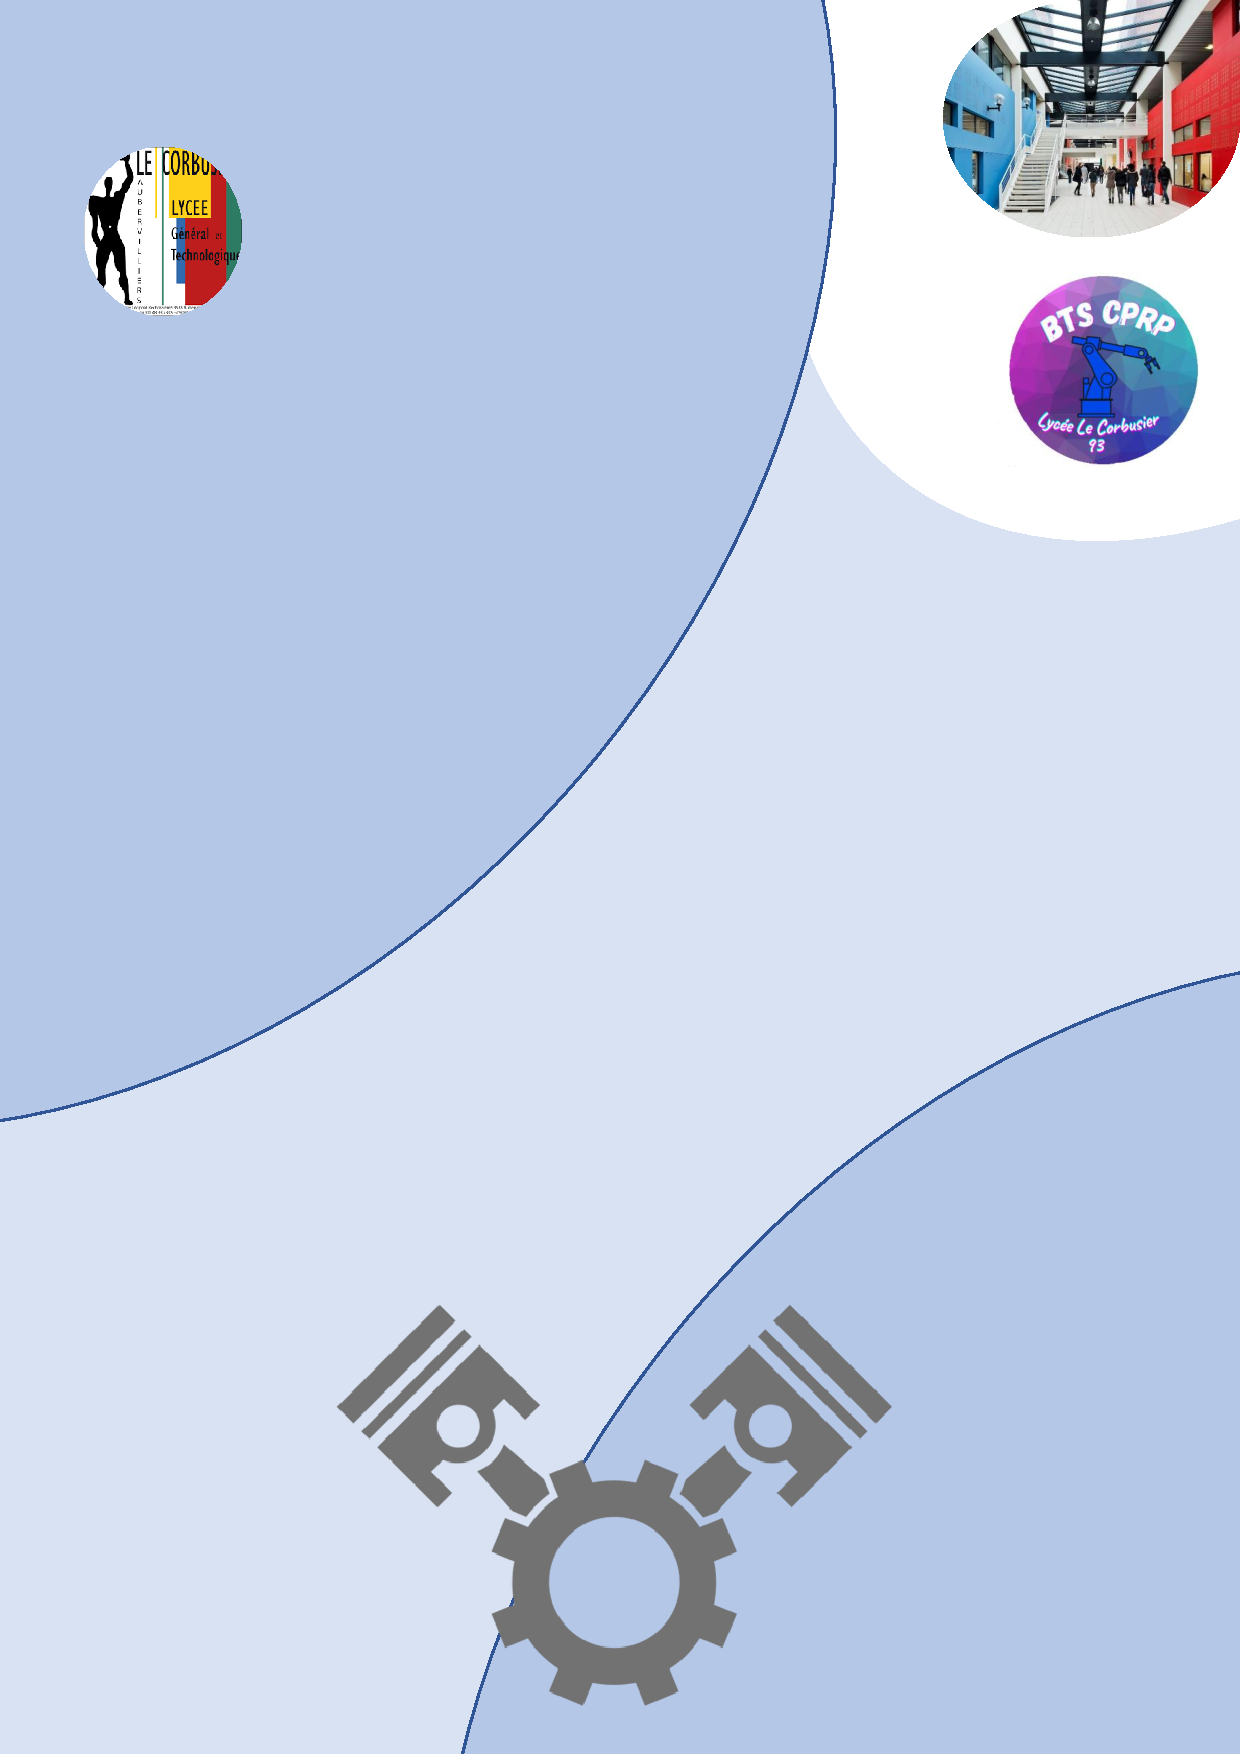
\includegraphics[width=\paperwidth]{background.pdf}} % Code to output the background image, which should be the same dimensions as the paper to fill the page entirely; leave empty for no background image
	{ % Title(s) and author(s)
		\centering\sffamily % Font styling
		{\Huge\bfseries Cours de conception préliminaire pour BTS CPRP\\ Sciences industrielles de l'ingénieur\par} % Book title
		\vspace{16pt} % Vertical whitespace
		{\LARGE Guide pratique\par} % Subtitle
		\vspace{24pt} % Vertical whitespace
		{\huge\bfseries \par} % Author name
	}

%----------------------------------------------------------------------------------------
%	COPYRIGHT PAGE
%----------------------------------------------------------------------------------------

\thispagestyle{empty} % Suppress headers and footers on this page

~\vfill % Push the text down to the bottom of the page

\noindent Copyright \copyright\ 2022 Vincent Chevalier\\ % Copyright notice

\noindent \textsc{Published by \LaTeX OverLeaf}\\ % Publisher

\noindent \textsc{\href{https://www.latextemplates.com/template/legrand-orange-book}{book-website.com}}\\ % URL
\noindent
Crédit : Template original codé par Vel Gayevskiy (vel@latextemplates.com) et Mathias Legrand (legrand.mathias@gmail.com). Sous licence Creative Commons Attribution-NonCommercial 4.0 License (la "Licence"). Vous ne pouvez utiliser ce fichier qu'en conformité avec la Licence. Vous pouvez obtenir une copie de la Licence à l'adresse  \url{https://creativecommons.org/licenses/by-nc-sa/4.0}. À moins que la loi applicable ne l'exige ou que cela ne fasse l'objet d'un accord écrit, le logiciel distribué sous la Licence est distribué sur une base \textsc{``en l'état'', sans garantie ni condition d'aucune sorte}, expresse ou implicite. Voir la Licence pour les termes spécifiques régissant les permissions et les limitations de la Licence.\\ % License information, replace this with your own license (if any)

\noindent \textit{First printing, n/a} % Printing/edition date

%----------------------------------------------------------------------------------------
%	TABLE OF CONTENTS
%----------------------------------------------------------------------------------------

\pagestyle{empty} % Disable headers and footers for the following pages

\tableofcontents % Output the table of contents

\listoffigures % Output the list of figures, comment or remove this command if not required

\listoftables % Output the list of tables, comment or remove this command if not required

\pagestyle{fancy} % Enable default headers and footers again

\cleardoublepage % Start the following content on a new page

%----------------------------------------------------------------------------------------
%	PART
%----------------------------------------------------------------------------------------

\part{Communiquer dans l'industrie}

%----------------------------------------------------------------------------------------
%	SECTIONING EXAMPLES CHAPTER
%----------------------------------------------------------------------------------------

\chapterimage{orange2.jpg} % Chapter heading image
\chapterspaceabove{6.75cm} % Whitespace from the top of the page to the chapter title on chapter pages
\chapterspacebelow{7.25cm} % Amount of vertical whitespace from the top margin to the start of the text on chapter pages

%------------------------------------------------

\chapter{Décrypter le dessin de définition}\index{Sectioning}
\begin{corollary}[S2.4] 
Représentations graphiques dérivées des maquettes numériques
\end{corollary}


\section{Les normes}\index{Sectioning!Sections}
\begin{definition}{Normes}

    La normalisation a pour objet de fournir des documents de référence portant sur des règles, des caractéristiques, des recommandations ou des exemples de bonnes pratiques, relatives à des produits, à des services, à des méthodes, à des processus ou à des organisations.\\ \textit{https://www.entreprises.gouv.fr/}
\end{definition}

\begin{figure}[H] % Use [H] to suppress floating and place the figure/table exactly where it is specified in the text
	\centering % Horizontally center the figure on the page
	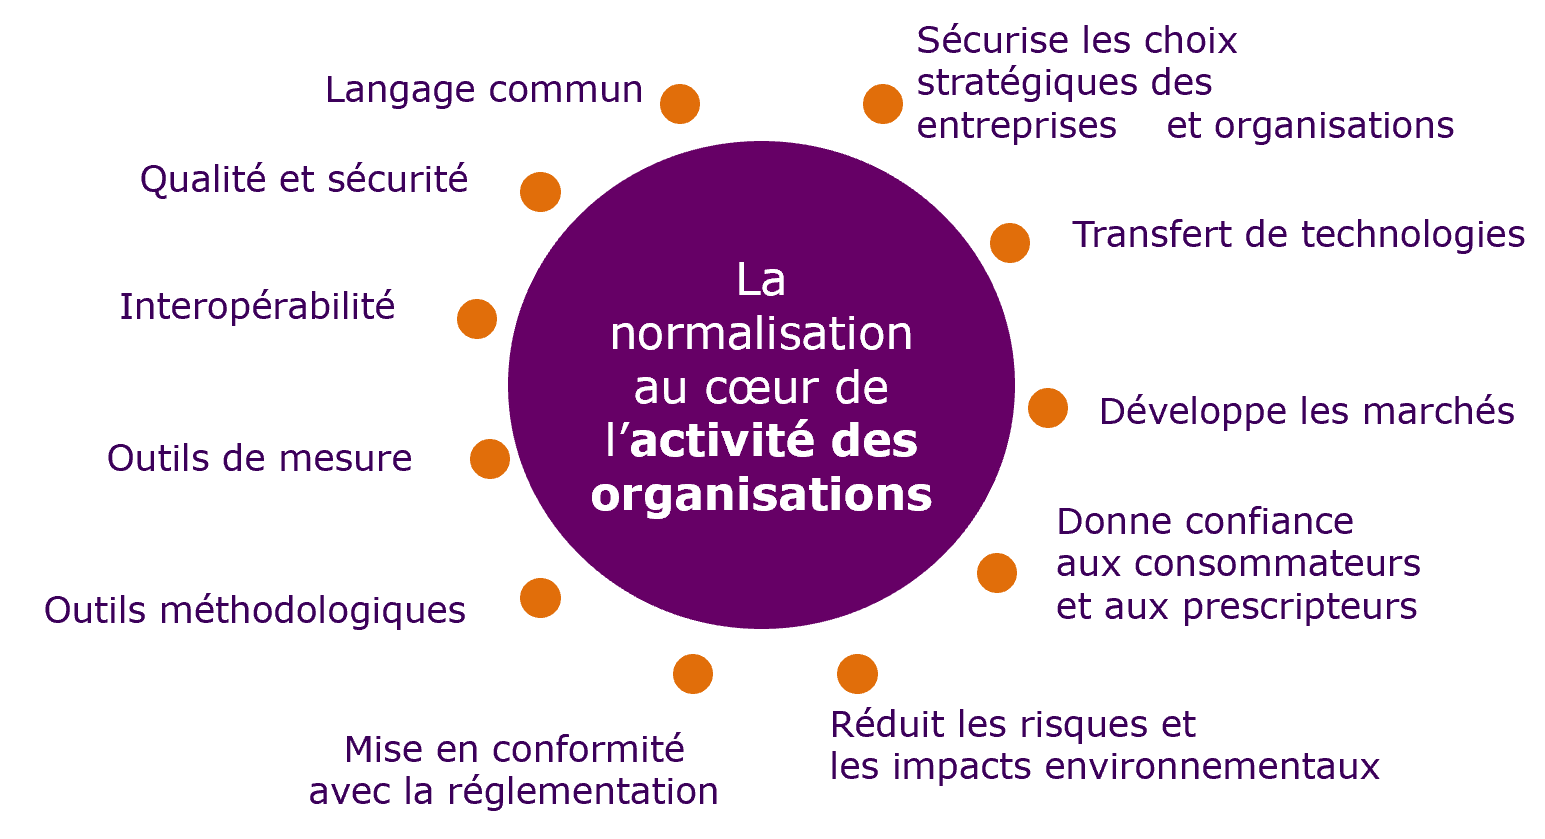
\includegraphics[width=0.7\textwidth]{normes.PNG} % Include the figure image
	\caption{AFNOR Nomarlisation}
	\label{fig:placeholder} % Unique label used for referencing the figure in-text
\end{figure}

Ces normes sont révisées régulièrement de façon à prendre en compte l’évolution de l’état de l’art. Ainsi, les entreprises y trouvent des solutions à des problèmes répétitifs, une actualisation permanente de l'état de l'art et des techniques. Elles contribuent également à la bonne communication entre les entreprise pour qu'elle puisse se comprendre.

Les normes à connaître :
\begin{itemize}
    \item ISO 9001 : définit les critères applicables à un système de management de la qualité. Il s’agit de la seule norme de la famille ISO 9000 à pouvoir être utilisée pour la certification (mais ce n’est pas une obligation);
    \item AFNOR NF Z 68-020 : Dénomination des axes pour les machines possédant 3 axes orthogonaux.
\end{itemize}

\section{Qu'est ce qu'un dessin de définition}\index{Sectioning!Subsections}
\subsection{Mise en plan d'une pièce}
Lorem ipsum dolor sit amet, consectetur adipiscing elit\footnote{Footnote example tos. Pellentesque iaculis odio vel nisl ullamcorper, nec faucibus ipsum molestie.}. Praesent porttitor arcu luctus, imperdiet urna iaculis, mattis eros. Pellentesque iaculis odio vel nisl ullamcorper.
\subsection{Les vues}
Lorem ipsum dolor sit amet, consectetur adipiscing elit Praesent porttitor arcu luctus, imperdiet urna iaculis, mattis eros. Pellentesque iaculis odio vel nisl ullamcorper.
\subsection{Les coupes}
Lorem ipsum dolor sit amet, consectetur adipiscing elit. Praesent porttitor arcu luctus, imperdiet urna iaculis, mattis eros. Pellentesque iaculis odio vel nisl ullamcorper.
\subsection{Les dimensions}
\begin{center}
  \begin{tikzpicture}
    \node (origin) at (0,0) {}; % shift relative baseline
    \coordinate (O) at (2,3);
    \draw[fill=gray!10] (O) circle (1);
    \draw[fill=blue!10] (2,4.5) ellipse (23pt and 16pt); %Entourer en bleu
    \draw[fill=red!10] (2.2,4.6) ellipse (13pt and 10pt); %Entourer en rouge
    \draw[fill=white] (O) circle (0.75) node[below,yshift=-1.125cm] {Un anneaux pour les gouverner tous};
    \draw[dim] (O) ++(-0.75,0) -- ++(1.5,0) node[midway,below] {$4^{\pm 0,5}$};
    \draw[dim] (O) ++(-1,1.25) -- ++(2,0) node[midway,above] {$5^{\pm 0,2}$}; 
    \foreach \x in {-1,1} {
      \draw (O) ++(\x,0.25) -- ++(0,1.25);
    }
    \end{tikzpicture}%
\end{center}

Une {\color{blue} spécification dimensionnelle} est une dimension exprimant une grandeur linéaire ou angulaire accompagnée d’un {\color{red}intervalle de tolérance} (ici $\pm 0,2$ et $\pm 0,5$ sont les intervalles de tolérance). Une {\color{red} cote} est une spécification dimensionnelle représentant la valeur de référence à laquelle s’ajoute l’intervalle de tolérance (IT).

  
La dimension réelle de chaque pièce doit se situer entre la valeur mini et la valeur maxi. En dehors de ces deux valeurs, la dimension est hors tolérance. 
\subsubsection{Côtes intrinsèques}
Une spécification intrinsèque est une spécification relative à une seule surface.


Fusce varius orci ac magna dapibus porttitor. In tempor leo a neque bibendum sollicitudin. Nulla pretium fermentum nisi, eget sodales magna facilisis eu. Praesent aliquet nulla ut bibendum lacinia. Donec vel mauris vulputate, commodo ligula ut, egestas orci. Suspendisse commodo odio sed hendrerit lobortis. Donec finibus eros erat, vel ornare enim mattis et. Donec finibus dolor quis dolor tempus consequat. Mauris fringilla dui id libero egestas, ut mattis neque ornare. Ut condimentum urna pharetra ipsum consequat, eu interdum elit cursus. Vivamus scelerisque tortor et nunc ultricies, id tincidunt libero pharetra. Aliquam eu imperdiet leo. Morbi a massa volutpat velit condimentum convallis et facilisis dolor.

In hac habitasse platea dictumst. Curabitur mattis elit sit amet justo luctus vestibulum. In hac habitasse platea dictumst. Pellentesque lobortis justo enim, a condimentum massa tempor eu. Ut quis nulla a quam pretium eleifend nec eu nisl. Nam cursus porttitor eros, sed luctus ligula convallis quis. Nam convallis, ligula in auctor euismod, ligula mauris fringilla tellus, et egestas mauris odio eget diam. Praesent sodales in ipsum eu dictum. Mauris interdum porttitor fringilla. Proin tincidunt sodales leo at ornare. Donec tempus magna non mauris gravida luctus. Cras vitae arcu vitae mauris eleifend scelerisque. Nam sem sapien, vulputate nec felis eu, blandit convallis risus. Pellentesque sollicitudin venenatis tincidunt. In et ipsum libero.

\subsubsection{Subsubsection Title} \index{Sectioning!Subsubsections}

Maecenas consectetur metus at tellus finibus condimentum. Proin arcu lectus, ultrices non tincidunt et, tincidunt ut quam. Integer luctus posuere est, non maximus ante dignissim quis. Nunc a cursus erat. Curabitur suscipit nibh in tincidunt sagittis. Nam malesuada vestibulum quam id gravida. Proin ut dapibus velit. Vestibulum eget quam quis ipsum semper convallis. Duis consectetur nibh ac diam dignissim, id condimentum enim dictum. Nam aliquet ligula eu magna pellentesque, nec sagittis leo lobortis. Aenean tincidunt dignissim egestas. Morbi efficitur risus ante, id tincidunt odio pulvinar vitae.

\paragraph{Paragraph Title}\index{Sectioning!Paragraphs} Nullam mollis tellus lorem, sed congue ipsum euismod a. Donec pulvinar neque sed ligula ornare sodales. Nulla sagittis vel lectus nec laoreet. Nulla volutpat malesuada turpis at ultricies. Ut luctus velit odio, sagittis volutpat erat aliquet vel. Donec ac neque eget neque volutpat mollis. Vestibulum viverra ligula et sapien bibendum, vel vulputate ex euismod. Curabitur nec velit velit. Aliquam vulputate lorem elit, id tempus nisl finibus sit amet. Curabitur ex turpis, consequat at lectus id, imperdiet molestie augue. Curabitur eu eros molestie purus commodo hendrerit. Quisque auctor ipsum nec mauris malesuada, non fringilla nibh viverra. Quisque gravida, metus quis semper pulvinar, dolor nisl suscipit leo, vestibulum volutpat ante justo ultrices diam. Sed id facilisis turpis, et aliquet eros.

In malesuada ullamcorper urna, sed dapibus diam sollicitudin non. Donec elit odio, accumsan ac nisl a, tempor imperdiet eros. Donec porta tortor eu risus consequat, a pharetra tortor tristique. Morbi sit amet laoreet erat. Morbi et luctus diam, quis porta ipsum. Quisque libero dolor, suscipit id facilisis eget, sodales volutpat dolor. Nullam vulputate interdum aliquam. Mauris id convallis erat, ut vehicula neque. Sed auctor nibh et elit fringilla, nec ultricies dui sollicitudin. Vestibulum vestibulum luctus metus venenatis facilisis. Suspendisse iaculis augue at vehicula ornare. Sed vel eros ut velit fermentum porttitor sed sed massa. Fusce venenatis, metus a rutrum sagittis, enim ex maximus velit, id semper nisi velit eu purus.

%------------------------------------------------

\section*{Unnumbered Section}

\subsection*{Unnumbered Subsection}

\subsubsection*{Unnumbered Subsubsection}

%----------------------------------------------------------------------------------------
%	IN-TEXT ELEMENT EXAMPLES CHAPTER
%----------------------------------------------------------------------------------------

\chapter{Nécessité de spécifications géométriques sur les plans}
\begin{corollary}[S6.1]
Spécification des produits
\end{corollary}

En plus des spécifications dimensionnelles, il est nécessaire d’indiquer des spécifications géométriques pour optimiser le montage ou le fonctionnement global d’un mécanisme.
Prenons l’exemple du rangement des pièces étalons dans leur boîte. La pièce 2 que l’on veut fabriquer a une dimension tolérancée de 20 h6.
On remarque que les surfaces 1 et 2 doivent être perpendiculaires, sinon la pièce ne rentrera peut-être pas. Le technicien a bien fabriqué la pièce à la dimension voulue, mais la pièce possède un défaut géométrique entre les surfaces 1 et 2 (défaut de perpendicularité).

\section{Symboles des spécifications géométriques}\index{Citation}

This statement requires citation \cite{Smith:2022jd}; this one is more specific \cite[162]{Smith:2021qr}.

%------------------------------------------------

\section{Link Examples}\index{Links}

This is a URL link: \href{https://www.latextemplates.com}{LaTeX Templates}. This is an email link: \href{mailto:example@example.com}{example@example.com}. This is a monospaced URL link: \url{https://www.LaTeXTemplates.com}.

%------------------------------------------------

\section{Lists}\index{Lists}

Lists are useful to present information in a concise and/or ordered way.

\subsection{Numbered List}\index{Lists!Numbered List}

\begin{enumerate}
	\item First numbered item
	\begin{enumerate}
		\item First indented numbered item
		\item Second indented numbered item
		\begin{enumerate}
			\item First second-level indented numbered item
		\end{enumerate}
	\end{enumerate}
	\item Second numbered item
	\item Third numbered item
\end{enumerate}

\subsection{Bullet Point List}\index{Lists!Bullet Points}

\begin{itemize}
	\item First bullet point item
	\begin{itemize}
		\item First indented bullet point item
		\item Second indented bullet point item
		\begin{itemize}
			\item First second-level indented bullet point item
		\end{itemize}
	\end{itemize}
	\item Second bullet point item
	\item Third bullet point item
\end{itemize}

\subsection{Descriptions and Definitions}\index{Lists!Descriptions and Definitions}

\begin{description}
	\item[Name] Description
	\item[Word] Definition
	\item[Comment] Elaboration
\end{description}

%------------------------------------------------

\section{International Support}

àáâäãåèéêëìíîïòóôöõøùúûüÿýñçčšž

\noindent ÀÁÂÄÃÅÈÉÊËÌÍÎÏÒÓÔÖÕØÙÚÛÜŸÝÑ

\noindent ßÇŒÆČŠŽ

%------------------------------------------------

\section{Ligatures}

fi fj fl ffl ffi Ty

%----------------------------------------------------------------------------------------
%	PART
%----------------------------------------------------------------------------------------

\part{Pourquoi ça casse ?}

%----------------------------------------------------------------------------------------
%	MATHEMATICS EXAMPLES CHAPTER
%----------------------------------------------------------------------------------------

\chapter{Dessiner des mécanismes}
\begin{corollary}[S3.1.1]
Cinématique des liaisons mécaniques
\end{corollary}



\section{Paramétrer les mécanismes}\index{Theorems}
Pour pouvoir analyser la structure d’un mécanisme, il est nécessaire de comprendre la description géométrique qui en est donnée, la plupart du temps, sous forme de schémas plus ou moins détaillés.
  \begin{center}
% Gradient Info
  
\tikzset {_gy0tq44fg/.code = {\pgfsetadditionalshadetransform{ \pgftransformshift{\pgfpoint{89.1 bp } { -128.7 bp }  }  \pgftransformscale{1.32 }  }}}
\pgfdeclareradialshading{_kahevi4yp}{\pgfpoint{-72bp}{104bp}}{rgb(0bp)=(1,1,1);
rgb(0bp)=(1,1,1);
rgb(25bp)=(0.48,0.15,0.15);
rgb(400bp)=(0.48,0.15,0.15)}
\tikzset{every picture/.style={line width=0.75pt}} %set default line width to 0.75pt        

\begin{tikzpicture}[x=0.75pt,y=0.75pt,yscale=-1,xscale=1]
%uncomment if require: \path (0,270); %set diagram left start at 0, and has height of 270

%Straight Lines [id:da3611151357134459] 
\draw [color={rgb, 255:red, 155; green, 155; blue, 155 }  ,draw opacity=1 ]   (117,173) -- (117,50) -- (117,47) ;
\draw [shift={(117,44)}, rotate = 90] [fill={rgb, 255:red, 155; green, 155; blue, 155 }  ,fill opacity=1 ][line width=0.08]  [draw opacity=0] (8.93,-4.29) -- (0,0) -- (8.93,4.29) -- cycle    ;
%Straight Lines [id:da3497273530839622] 
\draw [color={rgb, 255:red, 155; green, 155; blue, 155 }  ,draw opacity=1 ]   (117,173) -- (203.07,192.34) ;
\draw [shift={(206,193)}, rotate = 192.67] [fill={rgb, 255:red, 155; green, 155; blue, 155 }  ,fill opacity=1 ][line width=0.08]  [draw opacity=0] (8.93,-4.29) -- (0,0) -- (8.93,4.29) -- cycle    ;
%Straight Lines [id:da5086674449896322] 
\draw [color={rgb, 255:red, 155; green, 155; blue, 155 }  ,draw opacity=1 ]   (117,173) -- (52.97,246.73) ;
\draw [shift={(51,249)}, rotate = 310.97] [fill={rgb, 255:red, 155; green, 155; blue, 155 }  ,fill opacity=1 ][line width=0.08]  [draw opacity=0] (8.93,-4.29) -- (0,0) -- (8.93,4.29) -- cycle    ;
%Straight Lines [id:da6366387881571676] 
\draw [color={rgb, 255:red, 74; green, 144; blue, 226 }  ,draw opacity=1 ]   (117.29,89.5) -- (117,173) (121.26,99.52) -- (113.26,99.49)(121.22,109.52) -- (113.22,109.49)(121.19,119.52) -- (113.19,119.49)(121.15,129.52) -- (113.15,129.49)(121.12,139.52) -- (113.12,139.49)(121.08,149.52) -- (113.08,149.49)(121.05,159.52) -- (113.05,159.49)(121.01,169.52) -- (113.01,169.49) ;
%Straight Lines [id:da3121110592117222] 
\draw [color={rgb, 255:red, 155; green, 155; blue, 155 }  ,draw opacity=1 ] [dash pattern={on 4.5pt off 4.5pt}]  (145.9,132.8) -- (145.9,195.02) ;
%Straight Lines [id:da6429071342217672] 
\draw [color={rgb, 255:red, 155; green, 155; blue, 155 }  ,draw opacity=1 ] [dash pattern={on 4.5pt off 4.5pt}]  (173.9,89.7) -- (145.9,121.9) ;
%Straight Lines [id:da6669821751953844] 
\draw [color={rgb, 255:red, 155; green, 155; blue, 155 }  ,draw opacity=1 ] [dash pattern={on 4.5pt off 4.5pt}]  (80.9,108.08) -- (145.9,121.9) ;
%Shape: Right Angle [id:dp5978840607570464] 
\draw  [color={rgb, 255:red, 208; green, 2; blue, 27 }  ,draw opacity=1 ] (117,173) -- (117.29,89.5) -- (173.9,89.7) ;
%Shape: Circle [id:dp10467498350028093] 
\path  [shading=_kahevi4yp,_gy0tq44fg] (135,121.9) .. controls (135,115.88) and (139.88,111) .. (145.9,111) .. controls (151.92,111) and (156.8,115.88) .. (156.8,121.9) .. controls (156.8,127.92) and (151.92,132.8) .. (145.9,132.8) .. controls (139.88,132.8) and (135,127.92) .. (135,121.9) -- cycle ; % for fading 
 \draw   (135,121.9) .. controls (135,115.88) and (139.88,111) .. (145.9,111) .. controls (151.92,111) and (156.8,115.88) .. (156.8,121.9) .. controls (156.8,127.92) and (151.92,132.8) .. (145.9,132.8) .. controls (139.88,132.8) and (135,127.92) .. (135,121.9) -- cycle ; % for border 

%Straight Lines [id:da217119608671813] 
\draw [color={rgb, 255:red, 208; green, 2; blue, 27 }  ,draw opacity=1 ]   (117,173) -- (154,182) -- (146.33,195.02) ;
%Shape: Ellipse [id:dp435439963545865] 
\draw  [draw opacity=0][fill={rgb, 255:red, 0; green, 0; blue, 0 }  ,fill opacity=1 ][blur shadow={shadow xshift=0pt,shadow yshift=0pt, shadow blur radius=7.5pt, shadow blur steps=10 ,shadow opacity=100}] (145.96,187.67) .. controls (150.51,184.87) and (154.37,185.89) .. (154.57,189.95) .. controls (154.78,194.01) and (151.26,199.57) .. (146.7,202.37) .. controls (142.15,205.17) and (138.29,204.15) .. (138.09,200.09) .. controls (137.88,196.04) and (141.41,190.47) .. (145.96,187.67) -- cycle ;
%Straight Lines [id:da8673122096020862] 
\draw [color={rgb, 255:red, 208; green, 2; blue, 27 }  ,draw opacity=1 ]   (117,173) -- (81,216) -- (80.9,108.08) ;
%Straight Lines [id:da4638102219882483] 
\draw [color={rgb, 255:red, 74; green, 144; blue, 226 }  ,draw opacity=1 ]   (117,173) -- (81,216) (113.65,183.24) -- (107.51,178.1)(107.23,190.9) -- (101.09,185.77)(100.81,198.57) -- (94.67,193.43)(94.39,206.24) -- (88.26,201.1)(87.97,213.91) -- (81.84,208.77) ;
%Straight Lines [id:da354662584896545] 
\draw [color={rgb, 255:red, 74; green, 144; blue, 226 }  ,draw opacity=1 ]   (117,173) -- (154,182) (127.66,171.48) -- (125.77,179.25)(137.38,173.84) -- (135.49,181.61)(147.1,176.2) -- (145.2,183.98) ;
%Shape: Ellipse [id:dp8288820376151085] 
\draw  [draw opacity=0][fill={rgb, 255:red, 0; green, 0; blue, 0 }  ,fill opacity=1 ][blur shadow={shadow xshift=0pt,shadow yshift=0pt, shadow blur radius=7.5pt, shadow blur steps=10 ,shadow opacity=100}] (84.97,99.78) .. controls (89.74,99.57) and (91.78,103.11) .. (89.52,107.69) .. controls (87.27,112.27) and (81.59,116.16) .. (76.82,116.37) .. controls (72.06,116.58) and (70.02,113.04) .. (72.27,108.46) .. controls (74.53,103.88) and (80.21,99.99) .. (84.97,99.78) -- cycle ;
%Shape: Circle [id:dp48781094856000173] 
\draw  [draw opacity=0][fill={rgb, 255:red, 0; green, 0; blue, 0 }  ,fill opacity=1 ][blur shadow={shadow xshift=0pt,shadow yshift=0pt, shadow blur radius=6.75pt, shadow blur steps=9 ,shadow opacity=100}] (162.4,89.7) .. controls (162.4,83.35) and (167.55,78.2) .. (173.9,78.2) .. controls (180.25,78.2) and (185.4,83.35) .. (185.4,89.7) .. controls (185.4,96.05) and (180.25,101.2) .. (173.9,101.2) .. controls (167.55,101.2) and (162.4,96.05) .. (162.4,89.7) -- cycle ;
%Straight Lines [id:da4214282228187489] 
\draw [color={rgb, 255:red, 74; green, 144; blue, 226 }  ,draw opacity=1 ]   (279,109) -- (279,171) (283,119) -- (275,119)(283,129) -- (275,129)(283,139) -- (275,139)(283,149) -- (275,149)(283,159) -- (275,159)(283,169) -- (275,169) ;
%Shape: Circle [id:dp8470555363866257] 
\draw  [draw opacity=0][fill={rgb, 255:red, 0; green, 0; blue, 0 }  ,fill opacity=1 ][blur shadow={shadow xshift=0pt,shadow yshift=0pt, shadow blur radius=6.75pt, shadow blur steps=9 ,shadow opacity=100}] (437.4,142.7) .. controls (437.4,136.35) and (442.55,131.2) .. (448.9,131.2) .. controls (455.25,131.2) and (460.4,136.35) .. (460.4,142.7) .. controls (460.4,149.05) and (455.25,154.2) .. (448.9,154.2) .. controls (442.55,154.2) and (437.4,149.05) .. (437.4,142.7) -- cycle ;
%Shape: Axis 2D [id:dp6709157658899703] 
\draw [color={rgb, 255:red, 155; green, 155; blue, 155 }  ,draw opacity=1 ] (548.4,176.56) -- (576.6,176.56)(551.22,151) -- (551.22,179.4) (569.6,171.56) -- (576.6,176.56) -- (569.6,181.56) (546.22,158) -- (551.22,151) -- (556.22,158)  ;
\draw   ;

% Text Node
\draw (196,167.4) node [anchor=north west][inner sep=0.75pt]  [color={rgb, 255:red, 155; green, 155; blue, 155 }  ,opacity=1 ]  {$\vec{x}$};
% Text Node
\draw (123,37.4) node [anchor=north west][inner sep=0.75pt]  [color={rgb, 255:red, 155; green, 155; blue, 155 }  ,opacity=1 ]  {$\vec{y}$};
% Text Node
\draw (33,227.4) node [anchor=north west][inner sep=0.75pt]  [color={rgb, 255:red, 155; green, 155; blue, 155 }  ,opacity=1 ]  {$\vec{z}$};
% Text Node
\draw (130,156) node [anchor=north west][inner sep=0.75pt]  [color={rgb, 255:red, 74; green, 144; blue, 226 }  ,opacity=1 ] [align=left] {x};
% Text Node
\draw (100,120) node [anchor=north west][inner sep=0.75pt]  [color={rgb, 255:red, 74; green, 144; blue, 226 }  ,opacity=1 ] [align=left] {y};
% Text Node
\draw (104,190) node [anchor=north west][inner sep=0.75pt]  [color={rgb, 255:red, 74; green, 144; blue, 226 }  ,opacity=1 ] [align=left] {z};
% Text Node
\draw (363,29) node [anchor=north west][inner sep=0.75pt]   [align=left] {Légende :};
% Text Node
\draw (282.38,86.8) node  [font=\footnotesize] [align=left] {\begin{minipage}[lt]{78.04pt}\setlength\topsep{0pt}
\begin{center}
Longueur/coordonée\\sur l'axe
\end{center}

\end{minipage}};
% Text Node
\draw (345,121.4) node [anchor=north west][inner sep=0.75pt]  [color={rgb, 255:red, 155; green, 155; blue, 155 }  ,opacity=1 ]  {$\vec{x} ,\ \vec{y} ,\ \vec{z}$};
% Text Node
\draw (370.38,108.8) node  [font=\footnotesize] [align=left] {\begin{minipage}[lt]{16.78pt}\setlength\topsep{0pt}
\begin{center}
Axe
\end{center}

\end{minipage}};
% Text Node
\draw (279.38,190.8) node  [font=\footnotesize,color={rgb, 255:red, 74; green, 144; blue, 226 }  ,opacity=1 ] [align=left] {\begin{minipage}[lt]{23.42pt}\setlength\topsep{0pt}
\begin{center}
=\\x, y, z
\end{center}

\end{minipage}};
% Text Node
\draw (511.38,98.8) node  [font=\footnotesize] [align=left] {\begin{minipage}[lt]{83.67pt}\setlength\topsep{0pt}
\begin{center}
Projection de l'objet\\de l'espace sur le plan\\Exemple :
\end{center}

\end{minipage}};
% Text Node
\draw (527.38,140.8) node  [font=\footnotesize] [align=left] {\begin{minipage}[lt]{81.19pt}\setlength\topsep{0pt}
\begin{center}
Projection sur le plan 
\end{center}

\end{minipage}};
% Text Node
\draw (506,152.4) node [anchor=north west][inner sep=0.75pt]  [color={rgb, 255:red, 155; green, 155; blue, 155 }  ,opacity=1 ]  {$\vec{x} ,\ \vec{y}$};
% Connection
\draw    (360,48.83) .. controls (348.49,50.12) and (334.49,56.1) .. (318,66.76) ;
\draw [shift={(315.65,68.3)}, rotate = 326.42] [fill={rgb, 255:red, 0; green, 0; blue, 0 }  ][line width=0.08]  [draw opacity=0] (8.93,-4.29) -- (0,0) -- (8.93,4.29) -- cycle    ;
% Connection
\draw    (389.57,50) .. controls (380.22,63.89) and (374.46,79.19) .. (372.26,95.87) ;
\draw [shift={(371.91,98.8)}, rotate = 276.06] [fill={rgb, 255:red, 0; green, 0; blue, 0 }  ][line width=0.08]  [draw opacity=0] (8.93,-4.29) -- (0,0) -- (8.93,4.29) -- cycle    ;
% Connection
\draw    (434,47.73) .. controls (455.18,50.03) and (470.15,57.27) .. (478.94,69.41) ;
\draw [shift={(480.55,71.8)}, rotate = 237.93] [fill={rgb, 255:red, 0; green, 0; blue, 0 }  ][line width=0.08]  [draw opacity=0] (8.93,-4.29) -- (0,0) -- (8.93,4.29) -- cycle    ;

\end{tikzpicture}
\end{center}

Pour débuter, il vous faudra comprendre ce qu'est un repère et savoir les utiliser. Si vous regardez les sujets de BTS CPRP, vous verrez que la compréhension des repères sera utile pour avoir la bonne méthode de résolution des sujets.\\


Ici l'objet (une boule), à des coordonnées sur chaque axe. Si vous comptez le {\color{blue} nombre de trait} sur les axes, vous obtiendrez ses coordonnées\footnote{Les coordonnées sont les distances qui sépare l'objet de chaque axe, on regarde la distance entre l'objet et l'axe $\vec{x}$, puis la distance entre l'objet et l'axe $\vec{y}$, et enfin sur $\vec{z}$ par exemple.}. On le peut les noter sous en ligne ou en colonne.\\


Si on compte les traits (coordonnées) sur chaque axe par rapport à la boule, on a à peu près 3 et quelque sur l'axe $\vec{x}$, puis 5 et quelque sur l'axe $\vec{z}$ et enfin 8 et quelque sur $\vec{y}$. Si on veut noter ces informations en ligne, nous additionnerons les différentes longueurs, en précisant à chaque fois le nom de l'axe. Pour écrire les coordonnées en colonne, vous verrez certainement que le nom des axes n'est pas noté. Mais il convient de le préciser, surtout au début. Dans les deux cas, nous obtiendrons les notations suivantes :

\begin{center}
    

En ligne : Coordonnées de l'objet = $3\vec{x} + 8\vec{y} + 5\vec{z}$ \\
En colonne : Coordonnées de l'objet = $ \left\{ \begin{array}{c}
     3 \\
     8 \\
     5
\end{array} \right\} _{\vec{x}, \vec{y}, \vec{z}}$
\end{center}

\begin{remark}
    En fait, mathématiquement, pour calculer la longueur entre l'objet et les axes, on multiplie la longueur x (ici 3, 8 et 5) par le \textbf{vecteur unitaire} de l'axe. Pour être rigoureux, nous devrions dire ¨3 fois le vecteur unitaire de l'axe $\vec{x}$ ¨. Nous multiplions une longueur par une autre longueur, car le vecteur unitaire peut être 1. Si on parle en mètre, on aura 3 fois 1 mètre, ce qui donne 3 mètre. Comme ça, si on veut convertir le tout en feet (les unités de longueurs américaines), nous n'aurons pas à effectuer les conversion à chaque fois !
\end{remark}



\begin{exercise} % Specify a name/title in square brackets, or leave them out for no title
	Essayez de trouver les coordonnées des trois points suivants :
\end{exercise}


\tikzset{every picture/.style={line width=0.75pt}} %set default line width to 0.75pt        

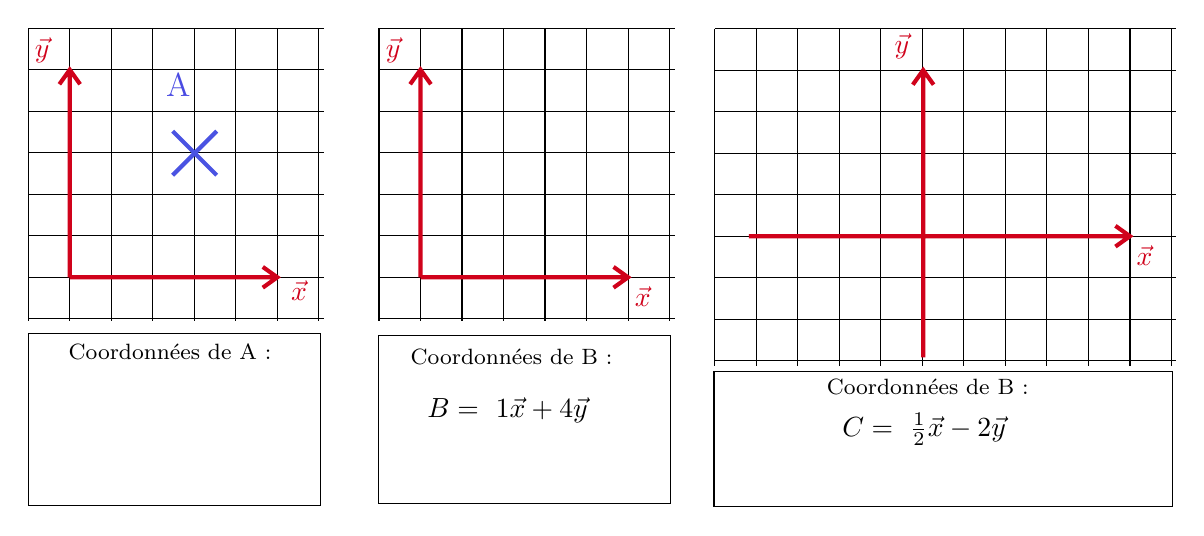
\begin{tikzpicture}[x=0.75pt,y=0.75pt,yscale=-1,xscale=1]
%uncomment if require: \path (0,321); %set diagram left start at 0, and has height of 321

%Shape: Grid [id:dp3932706137193831] 
\draw  [draw opacity=0] (90.2,40.2) -- (232.6,40.2) -- (232.6,181.2) -- (90.2,181.2) -- cycle ; \draw   (90.2,40.2) -- (90.2,181.2)(110.2,40.2) -- (110.2,181.2)(130.2,40.2) -- (130.2,181.2)(150.2,40.2) -- (150.2,181.2)(170.2,40.2) -- (170.2,181.2)(190.2,40.2) -- (190.2,181.2)(210.2,40.2) -- (210.2,181.2)(230.2,40.2) -- (230.2,181.2) ; \draw   (90.2,40.2) -- (232.6,40.2)(90.2,60.2) -- (232.6,60.2)(90.2,80.2) -- (232.6,80.2)(90.2,100.2) -- (232.6,100.2)(90.2,120.2) -- (232.6,120.2)(90.2,140.2) -- (232.6,140.2)(90.2,160.2) -- (232.6,160.2)(90.2,180.2) -- (232.6,180.2) ; \draw    ;
%Shape: Axis 2D [id:dp39250656962639074] 
\draw [color={rgb, 255:red, 208; green, 2; blue, 27 }  ,draw opacity=1 ][line width=1.5]  (110.2,160.2) -- (210.2,160.2)(110.2,60.2) -- (110.2,160.2) -- cycle (203.2,155.2) -- (210.2,160.2) -- (203.2,165.2) (105.2,67.2) -- (110.2,60.2) -- (115.2,67.2)  ;
\draw  [color={rgb, 255:red, 74; green, 83; blue, 226 }  ,draw opacity=1 ][line width=1.5]  (159.79,89.79) -- (181.01,111.01)(181.01,89.79) -- (159.79,111.01) ;
%Shape: Grid [id:dp9415796246319506] 
\draw  [draw opacity=0] (259.2,40.2) -- (401.6,40.2) -- (401.6,181.2) -- (259.2,181.2) -- cycle ; \draw   (259.2,40.2) -- (259.2,181.2)(279.2,40.2) -- (279.2,181.2)(299.2,40.2) -- (299.2,181.2)(319.2,40.2) -- (319.2,181.2)(339.2,40.2) -- (339.2,181.2)(359.2,40.2) -- (359.2,181.2)(379.2,40.2) -- (379.2,181.2)(399.2,40.2) -- (399.2,181.2) ; \draw   (259.2,40.2) -- (401.6,40.2)(259.2,60.2) -- (401.6,60.2)(259.2,80.2) -- (401.6,80.2)(259.2,100.2) -- (401.6,100.2)(259.2,120.2) -- (401.6,120.2)(259.2,140.2) -- (401.6,140.2)(259.2,160.2) -- (401.6,160.2)(259.2,180.2) -- (401.6,180.2) ; \draw    ;
%Shape: Axis 2D [id:dp2638809335795913] 
\draw [color={rgb, 255:red, 208; green, 2; blue, 27 }  ,draw opacity=1 ][line width=1.5]  (279.2,160.2) -- (379.2,160.2)(279.2,60.2) -- (279.2,160.2) -- cycle (372.2,155.2) -- (379.2,160.2) -- (372.2,165.2) (274.2,67.2) -- (279.2,60.2) -- (284.2,67.2)  ;
%Shape: Rectangle [id:dp783528924686701] 
\draw   (90.2,187.4) -- (230.8,187.4) -- (230.8,270) -- (90.2,270) -- cycle ;
%Shape: Rectangle [id:dp5161781809437043] 
\draw   (259,188.2) -- (399.6,188.2) -- (399.6,269.2) -- (259,269.2) -- cycle ;
%Shape: Grid [id:dp6409859497428556] 
\draw  [draw opacity=0] (421,40.4) -- (643,40.4) -- (643,202.8) -- (421,202.8) -- cycle ; \draw   (421,40.4) -- (421,202.8)(441,40.4) -- (441,202.8)(461,40.4) -- (461,202.8)(481,40.4) -- (481,202.8)(501,40.4) -- (501,202.8)(521,40.4) -- (521,202.8)(541,40.4) -- (541,202.8)(561,40.4) -- (561,202.8)(581,40.4) -- (581,202.8)(601,40.4) -- (601,202.8)(621,40.4) -- (621,202.8)(641,40.4) -- (641,202.8) ; \draw   (421,40.4) -- (643,40.4)(421,60.4) -- (643,60.4)(421,80.4) -- (643,80.4)(421,100.4) -- (643,100.4)(421,120.4) -- (643,120.4)(421,140.4) -- (643,140.4)(421,160.4) -- (643,160.4)(421,180.4) -- (643,180.4)(421,200.4) -- (643,200.4) ; \draw    ;
%Shape: Axis 2D [id:dp3605782735862748] 
\draw [color={rgb, 255:red, 208; green, 2; blue, 27 }  ,draw opacity=1 ][line width=1.5]  (437.4,140.4) -- (621,140.4)(521.4,60.4) -- (521.4,198.8) (614,135.4) -- (621,140.4) -- (614,145.4) (516.4,67.4) -- (521.4,60.4) -- (526.4,67.4)  ;
%Shape: Rectangle [id:dp30454929376549433] 
\draw   (420.6,205.8) -- (641.4,205.8) -- (641.4,270.8) -- (420.6,270.8) -- cycle ;

% Text Node
\draw (155.4,60.8) node [anchor=north west][inner sep=0.75pt]  [font=\large,color={rgb, 255:red, 74; green, 75; blue, 226 }  ,opacity=1 ] [align=left] {A};
% Text Node
\draw (108.4,191.2) node [anchor=north west][inner sep=0.75pt]  [font=\footnotesize] [align=left] {Coordonnées de A :};
% Text Node
\draw (273.2,193.6) node [anchor=north west][inner sep=0.75pt]  [font=\footnotesize] [align=left] {Coordonnées de B :};
% Text Node
\draw (281.2,216.8) node [anchor=north west][inner sep=0.75pt]    {$B=\ 1\vec{x} +4\vec{y}$};
% Text Node
\draw (473.7,208.07) node [anchor=north west][inner sep=0.75pt]  [font=\footnotesize] [align=left] {Coordonnées de B :};
% Text Node
\draw (481.13,224.2) node [anchor=north west][inner sep=0.75pt]    {$C=\ \frac{1}{2}\vec{x} -2\vec{y}$};
% Text Node
\draw (215.6,160.8) node [anchor=north west][inner sep=0.75pt]  [color={rgb, 255:red, 208; green, 2; blue, 27 }  ,opacity=1 ]  {$\vec{x}$};
% Text Node
\draw (381.2,163.6) node [anchor=north west][inner sep=0.75pt]  [color={rgb, 255:red, 208; green, 2; blue, 27 }  ,opacity=1 ]  {$\vec{x}$};
% Text Node
\draw (623,143.8) node [anchor=north west][inner sep=0.75pt]  [color={rgb, 255:red, 208; green, 2; blue, 27 }  ,opacity=1 ]  {$\vec{x}$};
% Text Node
\draw (506.4,41.4) node [anchor=north west][inner sep=0.75pt]  [color={rgb, 255:red, 208; green, 2; blue, 27 }  ,opacity=1 ]  {$\vec{y}$};
% Text Node
\draw (261.2,43.6) node [anchor=north west][inner sep=0.75pt]  [color={rgb, 255:red, 208; green, 2; blue, 27 }  ,opacity=1 ]  {$\vec{y}$};
% Text Node
\draw (92.2,43.6) node [anchor=north west][inner sep=0.75pt]  [color={rgb, 255:red, 208; green, 2; blue, 27 }  ,opacity=1 ]  {$\vec{y}$};


\end{tikzpicture}


\subsection{Several equations}\index{Theorems!Several Equations}

This is a theorem consisting of several equations.

\begin{theorem}[Name of the theorem] % Specify a name/title in square brackets, or leave them out for no title
	In $E=\mathbb{R}^n$ all norms are equivalent. It has the properties:
	\begin{align}
		& \big| ||\mathbf{x}|| - ||\mathbf{y}|| \big|\leq || \mathbf{x}- \mathbf{y}||\\
		&  ||\sum_{i=1}^n\mathbf{x}_i||\leq \sum_{i=1}^n||\mathbf{x}_i||\quad\text{where $n$ is a finite integer}
	\end{align}
\end{theorem}

\subsection{Single Line}\index{Theorems!Single Line}

This is a theorem consisting of just one line.

\begin{theorem} % Specify a name/title in square brackets, or leave them out for no title
	A set $\mathcal{D}(G)$ in dense in $L^2(G)$, $|\cdot|_0$. 
\end{theorem}

%------------------------------------------------

\section{Élaborer un schéma cinématique}\index{Definitions}

A definition can be mathematical or it could define a concept.

\begin{definition}[Definition name] % Specify a name/title in square brackets, or leave them out for no title
	Given a vector space $E$, a norm on $E$ is an application, denoted $||\cdot||$, $E$ in $\mathbb{R}^+=[0,+\infty[$ such that:
	\begin{align}
		& ||\mathbf{x}||=0\ \Rightarrow\ \mathbf{x}=\mathbf{0}\\
		& ||\lambda \mathbf{x}||=|\lambda|\cdot ||\mathbf{x}||\\
		& ||\mathbf{x}+\mathbf{y}||\leq ||\mathbf{x}||+||\mathbf{y}||
	\end{align}
\end{definition}

%------------------------------------------------

\section{Mouvement entre les solides}\index{Notations}
\begin{corollary}[S3] 
\begin{itemize}
    \item S3.2 Mouvements relatifs entre solides dans le cas d'une translation ou d'une rotation autour d'un axe fixe;
    \item S3.3 Mouvements plans.
\end{itemize}

\end{corollary}



\begin{notation} % Specify a name/title in square brackets, or leave them out for no title
	Given an open subset $G$ of $\mathbb{R}^n$, the set of functions $\varphi$ are:
	\begin{enumerate}
		\item Bounded support $G$;
		\item Infinitely differentiable;
	\end{enumerate}
	a vector space is denoted by $\mathcal{D}(G)$. 
\end{notation}

%------------------------------------------------

\section{Statisme d'un système}\index{Remarks}

This is an example of a remark.

$\{ \mathcal{V} (S/R) \}
= \left\{ \begin{array}{c}
     \overrightarrow{\Omega} (S/R) \\
     \overrightarrow{V} (B \in S/R)
\end{array} \right\} _{B/R}
= \left\{ \begin{array}{c}
     \overrightarrow{\Omega} (S/R) \\
     \overrightarrow{V} (A \in S/R) +\overrightarrow{BA} \wedge \overrightarrow{\Omega}(S/R)
\end{array} \right\} _{B/R}$

\begin{remark}
    On termine ce chapitre en éveillant le lecteur aux qualités respectives de l’isostatisme
et de l’hyperstatisme :

• pour une fonction mécanique souhaitée, une structure isostatique est plus écono-
mique qu’une structure hyperstatique ;

• une structure hyperstatique est plus rigide qu’une structure isostatique.

En effet, les contraintes géométriques mises en évidence dans le cas de l’hyperstatis-
me induisent soit une qualité de fabrication plus grande, soit la mise en place de

réglages sur le mécanisme. On sait tout à fait réaliser et l’un, et l’autre, mais cela a un
coût. En conclusion, on peut dire que l’hyperstatisme est un choix réfléchi qu’il est
nécessaire de financer quand les critères de performances ne sont pas atteints avec une
structure équivalente isostatique.
Chercher à rendre une structure isostatique est une activité qui sollicite l’imagination
et que l’on illustre sur un exemple.
\end{remark}

%------------------------------------------------

\section{Matériaux \& traitement}\index{Corollaries}
\begin{corollary}[S4.1]
Structure et caractéristiques des matériaux
\end{corollary}

%------------------------------------------------

\section{Propositions}\index{Propositions}

\subsection{Several equations}\index{Propositions!Several Equations}

\begin{proposition}[Proposition name] % Specify a name/title in square brackets, or leave them out for no title
	It has the properties:
	\begin{align}
		& \big| ||\mathbf{x}|| - ||\mathbf{y}|| \big|\leq || \mathbf{x}- \mathbf{y}||\\
		&  ||\sum_{i=1}^n\mathbf{x}_i||\leq \sum_{i=1}^n||\mathbf{x}_i||\quad\text{where $n$ is a finite integer}
	\end{align}
\end{proposition}

\subsection{Single Line}\index{Propositions!Single Line}

\begin{proposition} % Specify a name/title in square brackets, or leave them out for no title
	Let $f,g\in L^2(G)$; if $\forall \varphi\in\mathcal{D}(G)$, $(f,\varphi)_0=(g,\varphi)_0$ then $f = g$. 
\end{proposition}

%------------------------------------------------

\section{Examples}\index{Examples}

\subsection{Equation Example}\index{Examples!Equation}

\begin{example} % Specify a name/title in square brackets, or leave them out for no title
	Let $G=\{x\in\mathbb{R}^2:|x|<3\}$ and denoted by: $x^0=(1,1)$; consider the function:
	\begin{equation}
	f(x)=\left\{\begin{aligned} & \mathrm{e}^{|x|} & & \text{si $|x-x^0|\leq 1/2$}\\
	& 0 & & \text{si $|x-x^0|> 1/2$}\end{aligned}\right.
	\end{equation}
	The function $f$ has bounded support, we can take $A=\{x\in\mathbb{R}^2:|x-x^0|\leq 1/2+\epsilon\}$ for all $\epsilon\in\mathopen{]}0\,;5/2-\sqrt{2}\mathclose{[}$.
\end{example}

\subsection{Text Example}\index{Examples!Text}

\begin{example}[Example name] % Specify a name/title in square brackets, or leave them out for no title
	Aliquam arcu turpis, ultrices sed luctus ac, vehicula id metus. Morbi eu feugiat velit, et tempus augue. Proin ac mattis tortor. Donec tincidunt, ante rhoncus luctus semper, arcu lorem lobortis justo, nec convallis ante quam quis lectus. Aenean tincidunt sodales massa, et hendrerit tellus mattis ac. Sed non pretium nibh. Donec cursus maximus luctus. Vivamus lobortis eros et massa porta porttitor.
\end{example}

%------------------------------------------------

\section{Exercises}\index{Exercises}

\begin{exercise} % Specify a name/title in square brackets, or leave them out for no title
	This is a good place to ask a question to test learning progress or further cement ideas into students' minds.
\end{exercise}

%------------------------------------------------

\section{Problems}\index{Problems}

\begin{problem} % Specify a name/title in square brackets, or leave them out for no title
	What is the average airspeed velocity of an unladen swallow?
\end{problem}

%------------------------------------------------

\section{Vocabulary}\index{Vocabulary}

Define a word to improve a students' vocabulary.

\begin{vocabulary}[Word] % Specify a name/title in square brackets, or leave them out for no title
	Definition of word.
\end{vocabulary}




\part{Concevoir un produit}

%----------------------------------------------------------------------------------------
%	MATHEMATICS EXAMPLES CHAPTER
%----------------------------------------------------------------------------------------

\chapter{Gestion de projet}
\begin{corollary}[S1.3]
Compétitivité des produits industriels
\end{corollary}



%----------------------------------------------------------------------------------------
%	PRESENTING INFORMATION/RESULTS EXAMPLES CHAPTER
%----------------------------------------------------------------------------------------

\chapterimage{orange3.jpg} % Chapter heading image
\chapterspaceabove{6.25cm} % Whitespace from the top of the page to the chapter title on chapter pages
\chapterspacebelow{7.5cm} % Amount of vertical whitespace from the top margin to the start of the text on chapter pages

%------------------------------------------------

\chapter{Chapitre}

\begin{corollary}[S6.1]
Spécification des produits
\end{corollary}

\begin{table}[H] % Use [H] to suppress floating and place the figure/table exactly where it is specified in the text
	\centering % Horizontally center the table on the page
	\begin{tabular}{L{0.15\textwidth} R{0.15\textwidth} R{0.15\textwidth}} % Specify column alignment with L{width}, C{width} and R{width} for fixed-width columns, or the default latex l, c and r for flexible-width columns
		\toprule
		\textbf{Treatments} & \textbf{Response 1} & \textbf{Response 2}\\
		\midrule
		Treatment 1 & 0.0003262 & 0.562 \\
		Treatment 2 & 0.0015681 & 0.910 \\
		Treatment 3 & 0.0009271 & 0.296 \\
		\bottomrule
	\end{tabular}
	\caption{Table caption.}
	\label{tab:example} % Unique label used for referencing the table in-text
\end{table}

Referencing \autoref{tab:example} in-text using its label.

\begin{table}[t] % Floating table, [t] tells LaTeX to place it at the top of the next available page
	\centering % Horizontally center the table on the page
	\begin{tabular}{L{0.15\textwidth} R{0.15\textwidth} R{0.15\textwidth}} % Specify column alignment with L{width}, C{width} and R{width} for fixed-width columns, or the default latex l, c and r for flexible-width columns
		\toprule
		\textbf{Treatments} & \textbf{Response 1} & \textbf{Response 2}\\
		\midrule
		Treatment 1 & 0.0003262 & 0.562 \\
		Treatment 2 & 0.0015681 & 0.910 \\
		Treatment 3 & 0.0009271 & 0.296 \\
		\bottomrule
	\end{tabular}
	\caption{Floating table.}
	\label{tab:floating} % Unique label used for referencing the table in-text
\end{table}

%------------------------------------------------

\section{Figure}\index{Figure}

Lorem ipsum dolor sit amet, consectetur adipiscing elit. Praesent porttitor arcu luctus, imperdiet urna iaculis, mattis eros. Pellentesque iaculis odio vel nisl ullamcorper, nec faucibus ipsum molestie. Sed dictum nisl non aliquet porttitor. Etiam vulputate arcu dignissim, finibus sem et, viverra nisl. Aenean luctus congue massa, ut laoreet metus ornare in. Nunc fermentum nisi imperdiet lectus tincidunt vestibulum at ac elit. Nulla mattis nisl eu malesuada suscipit.

\begin{figure}[H] % Use [H] to suppress floating and place the figure/table exactly where it is specified in the text
	\centering % Horizontally center the figure on the page
	
\includegraphics[width=0.5\textwidth]{creodocs_logo.pdf} % Include the figure image
	\caption{Figure caption.}
	\label{fig:placeholder} % Unique label used for referencing the figure in-text
\end{figure}

Referencing \autoref{fig:placeholder} in-text using its label.

\begin{figure}[b] % Floating figure, [b] tells LaTeX to place it at the bottom of the next available page
	\centering % Horizontally center the figure on the page
	
\includegraphics[width=\textwidth]{creodocs_logo.pdf} % Include the figure image
	\caption{Floating figure.}
	\label{fig:floating} % Unique label used for referencing the figure in-text
\end{figure}

%----------------------------------------------------------------------------------------

\stopcontents[part] % Manually stop the 'part' table of contents here so the previous Part page table of contents doesn't list the following chapters

%----------------------------------------------------------------------------------------
%	BIBLIOGRAPHY
%----------------------------------------------------------------------------------------

\chapterimage{} % Chapter heading image
\chapterspaceabove{2.5cm} % Whitespace from the top of the page to the chapter title on chapter pages
\chapterspacebelow{2cm} % Amount of vertical whitespace from the top margin to the start of the text on chapter pages

%------------------------------------------------

\chapter*{Bibliography}
\markboth{\sffamily\normalsize\bfseries Bibliography}{\sffamily\normalsize\bfseries Bibliography} % Set the page headers to display a Bibliography chapter name
\addcontentsline{toc}{chapter}{\textcolor{black}{Bibliography}} % Add a Bibliography heading to the table of contents

\section*{Articles}
\addcontentsline{toc}{section}{Articles} % Add the Articles subheading to the table of contents

\printbibliography[heading=bibempty, type=article] % Output article bibliography entries

\section*{Books}
\addcontentsline{toc}{section}{Books} % Add the Books subheading to the table of contents

\printbibliography[heading=bibempty, type=book] % Output book bibliography entries

%----------------------------------------------------------------------------------------
%	INDEX
%----------------------------------------------------------------------------------------

\cleardoublepage % Make sure the index starts on an odd (right side) page
\phantomsection
\addcontentsline{toc}{chapter}{\textcolor{ocre}{Index}} % Add an Index heading to the table of contents
\printindex % Output the index

%----------------------------------------------------------------------------------------
%	APPENDICES
%----------------------------------------------------------------------------------------

\chapterimage{orange2.jpg} % Chapter heading image
\chapterspaceabove{6.75cm} % Whitespace from the top of the page to the chapter title on chapter pages
\chapterspacebelow{7.25cm} % Amount of vertical whitespace from the top margin to the start of the text on chapter pages

\begin{appendices}

\renewcommand{\chaptername}{Appendix} % Change the chapter name to Appendix, i.e. "Appendix A: Title", instead of "Chapter A: Title" in the headers

%------------------------------------------------

\chapter{Appendix Chapter Title}

\section{Appendix Section Title}

Lorem ipsum dolor sit amet, consectetur adipiscing elit. Aliquam auctor mi risus, quis tempor libero hendrerit at. Duis hendrerit placerat quam et semper. Nam ultricies metus vehicula arcu viverra, vel ullamcorper justo elementum. Pellentesque vel mi ac lectus cursus posuere et nec ex. Fusce quis mauris egestas lacus commodo venenatis. Ut at arcu lectus. Donec et urna nunc. Morbi eu nisl cursus sapien eleifend tincidunt quis quis est. Donec ut orci ex. Praesent ligula enim, ullamcorper non lorem a, ultrices volutpat dolor. Nullam at imperdiet urna. Pellentesque nec velit eget est euismod pretium.

%------------------------------------------------

\chapter{Appendix Chapter Title}

\section{Appendix Section Title}

Lorem ipsum dolor sit amet, consectetur adipiscing elit. Aliquam auctor mi risus, quis tempor libero hendrerit at. Duis hendrerit placerat quam et semper. Nam ultricies metus vehicula arcu viverra, vel ullamcorper justo elementum. Pellentesque vel mi ac lectus cursus posuere et nec ex. Fusce quis mauris egestas lacus commodo venenatis. Ut at arcu lectus. Donec et urna nunc. Morbi eu nisl cursus sapien eleifend tincidunt quis quis est. Donec ut orci ex. Praesent ligula enim, ullamcorper non lorem a, ultrices volutpat dolor. Nullam at imperdiet urna. Pellentesque nec velit eget est euismod pretium.

%------------------------------------------------

\end{appendices}

%----------------------------------------------------------------------------------------

\end{document}
